\documentclass[1p]{elsarticle_modified}
%\bibliographystyle{elsarticle-num}

%\usepackage[colorlinks]{hyperref}
%\usepackage{abbrmath_seonhwa} %\Abb, \Ascr, \Acal ,\Abf, \Afrak
\usepackage{amsfonts}
\usepackage{amssymb}
\usepackage{amsmath}
\usepackage{amsthm}
\usepackage{scalefnt}
\usepackage{amsbsy}
\usepackage{kotex}
\usepackage{caption}
\usepackage{subfig}
\usepackage{color}
\usepackage{graphicx}
\usepackage{xcolor} %% white, black, red, green, blue, cyan, magenta, yellow
\usepackage{float}
\usepackage{setspace}
\usepackage{hyperref}

\usepackage{tikz}
\usetikzlibrary{arrows}

\usepackage{multirow}
\usepackage{array} % fixed length table
\usepackage{hhline}

%%%%%%%%%%%%%%%%%%%%%
\makeatletter
\renewcommand*\env@matrix[1][\arraystretch]{%
	\edef\arraystretch{#1}%
	\hskip -\arraycolsep
	\let\@ifnextchar\new@ifnextchar
	\array{*\c@MaxMatrixCols c}}
\makeatother %https://tex.stackexchange.com/questions/14071/how-can-i-increase-the-line-spacing-in-a-matrix
%%%%%%%%%%%%%%%

\usepackage[normalem]{ulem}

\newcommand{\msout}[1]{\ifmmode\text{\sout{\ensuremath{#1}}}\else\sout{#1}\fi}
%SOURCE: \msout is \stkout macro in https://tex.stackexchange.com/questions/20609/strikeout-in-math-mode

\newcommand{\cancel}[1]{
	\ifmmode
	{\color{red}\msout{#1}}
	\else
	{\color{red}\sout{#1}}
	\fi
}

\newcommand{\add}[1]{
	{\color{blue}\uwave{#1}}
}

\newcommand{\replace}[2]{
	\ifmmode
	{\color{red}\msout{#1}}{\color{blue}\uwave{#2}}
	\else
	{\color{red}\sout{#1}}{\color{blue}\uwave{#2}}
	\fi
}

\newcommand{\Sol}{\mathcal{S}} %segment
\newcommand{\D}{D} %diagram
\newcommand{\A}{\mathcal{A}} %arc


%%%%%%%%%%%%%%%%%%%%%%%%%%%%%5 test

\def\sl{\operatorname{\textup{SL}}(2,\Cbb)}
\def\psl{\operatorname{\textup{PSL}}(2,\Cbb)}
\def\quan{\mkern 1mu \triangleright \mkern 1mu}

\theoremstyle{definition}
\newtheorem{thm}{Theorem}[section]
\newtheorem{prop}[thm]{Proposition}
\newtheorem{lem}[thm]{Lemma}
\newtheorem{ques}[thm]{Question}
\newtheorem{cor}[thm]{Corollary}
\newtheorem{defn}[thm]{Definition}
\newtheorem{exam}[thm]{Example}
\newtheorem{rmk}[thm]{Remark}
\newtheorem{alg}[thm]{Algorithm}

\newcommand{\I}{\sqrt{-1}}
\begin{document}

%\begin{frontmatter}
%
%\title{Boundary parabolic representations of knots up to 8 crossings}
%
%%% Group authors per affiliation:
%\author{Yunhi Cho} 
%\address{Department of Mathematics, University of Seoul, Seoul, Korea}
%\ead{yhcho@uos.ac.kr}
%
%
%\author{Seonhwa Kim} %\fnref{s_kim}}
%\address{Center for Geometry and Physics, Institute for Basic Science, Pohang, 37673, Korea}
%\ead{ryeona17@ibs.re.kr}
%
%\author{Hyuk Kim}
%\address{Department of Mathematical Sciences, Seoul National University, Seoul 08826, Korea}
%\ead{hyukkim@snu.ac.kr}
%
%\author{Seokbeom Yoon}
%\address{Department of Mathematical Sciences, Seoul National University, Seoul, 08826,  Korea}
%\ead{sbyoon15@snu.ac.kr}
%
%\begin{abstract}
%We find all boundary parabolic representation of knots up to 8 crossings.
%
%\end{abstract}
%\begin{keyword}
%    \MSC[2010] 57M25 
%\end{keyword}
%
%\end{frontmatter}

%\linenumbers
%\tableofcontents
%
\newcommand\colored[1]{\textcolor{white}{\rule[-0.35ex]{0.8em}{1.4ex}}\kern-0.8em\color{red} #1}%
%\newcommand\colored[1]{\textcolor{white}{ #1}\kern-2.17ex	\textcolor{white}{ #1}\kern-1.81ex	\textcolor{white}{ #1}\kern-2.15ex\color{red}#1	}

{\Large $\underline{12a_{1226}~(K12a_{1226})}$}

\setlength{\tabcolsep}{10pt}
\renewcommand{\arraystretch}{1.6}
\vspace{1cm}\begin{tabular}{m{100pt}>{\centering\arraybackslash}m{274pt}}
\multirow{5}{120pt}{
	\centering
	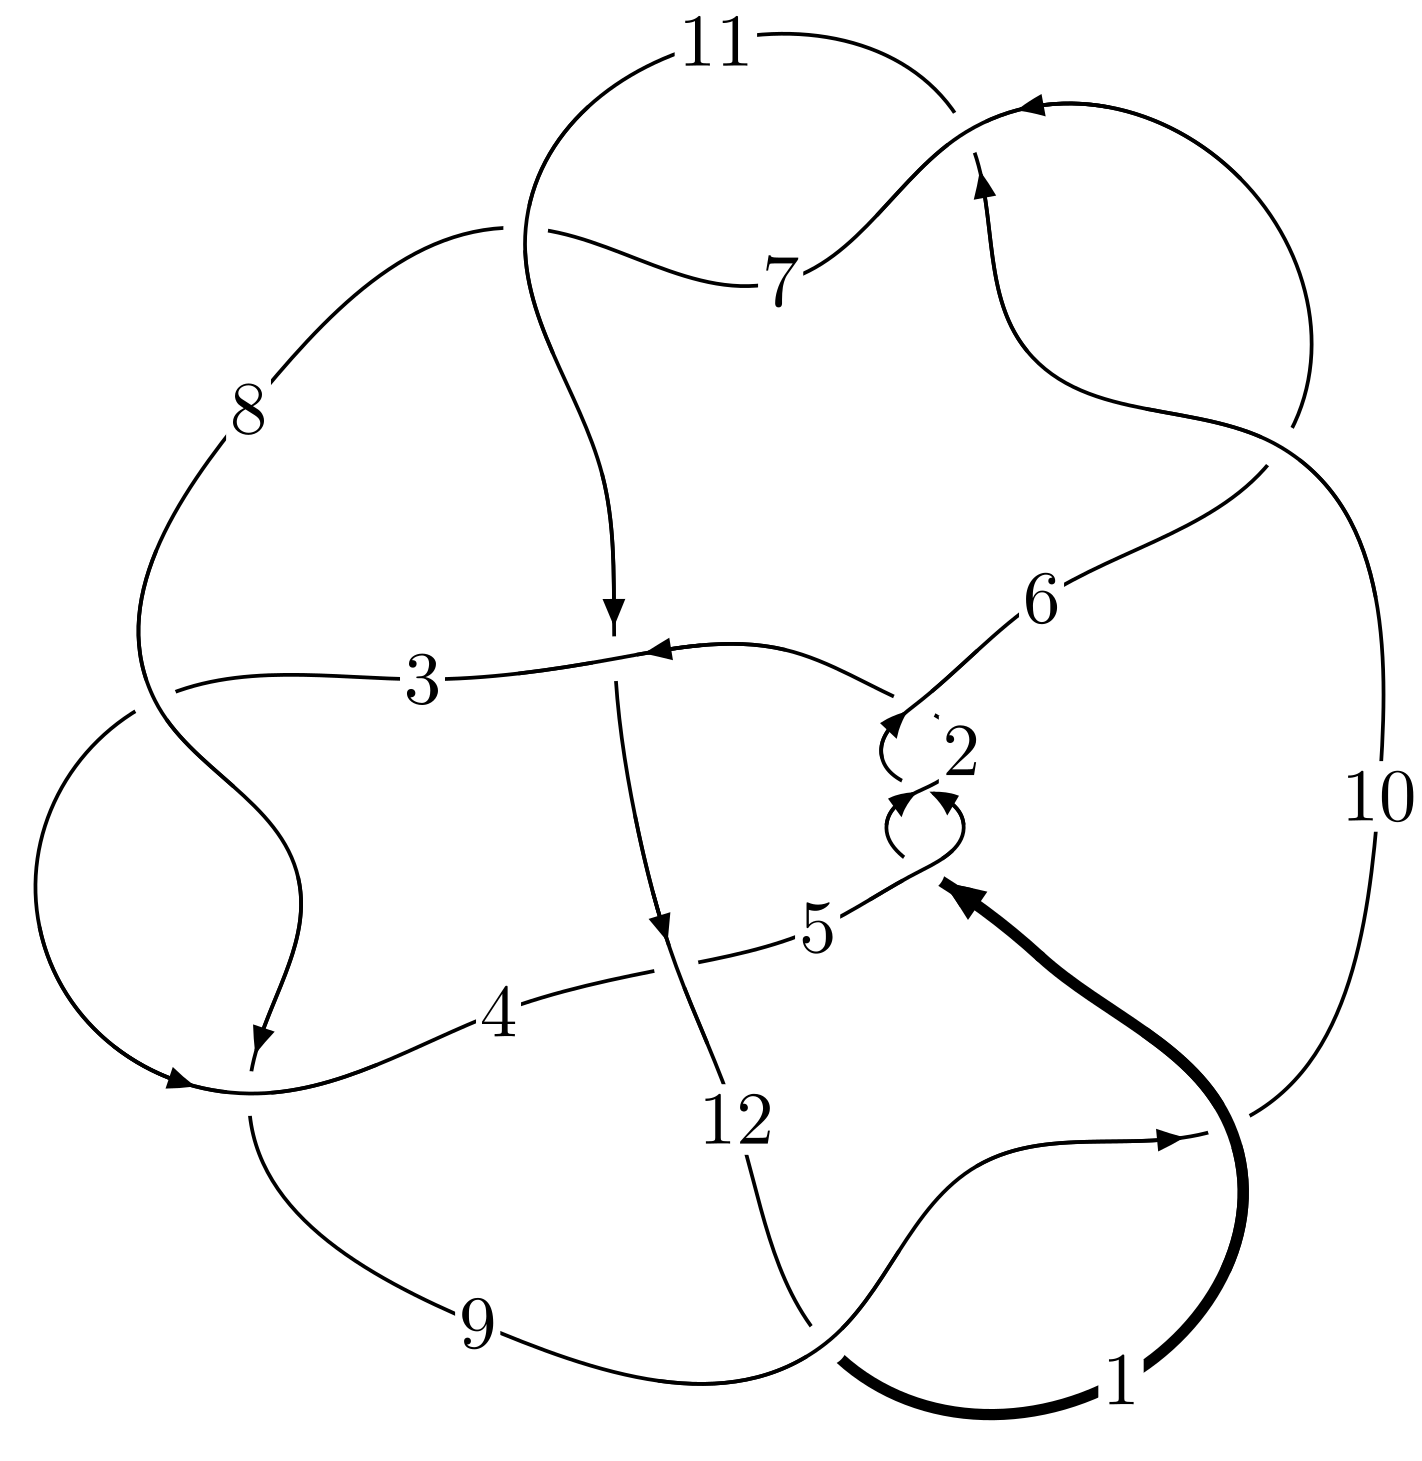
\includegraphics[width=112pt]{../../../GIT/diagram.site/Diagrams/png/2027_12a_1226.png}\\
\ \ \ A knot diagram\footnotemark}&
\allowdisplaybreaks
\textbf{Linearized knot diagam} \\
\cline{2-2}
 &
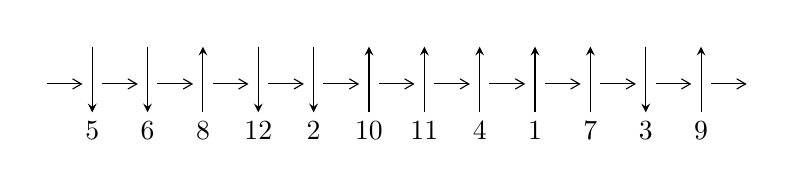
\begin{tikzpicture}[x=20pt, y=17pt]
	% nodes
	\node (C0) at (0, 0) {};
	\node (C1) at (1, 0) {};
	\node (C1U) at (1, +1) {};
	\node (C1D) at (1, -1) {5};

	\node (C2) at (2, 0) {};
	\node (C2U) at (2, +1) {};
	\node (C2D) at (2, -1) {6};

	\node (C3) at (3, 0) {};
	\node (C3U) at (3, +1) {};
	\node (C3D) at (3, -1) {8};

	\node (C4) at (4, 0) {};
	\node (C4U) at (4, +1) {};
	\node (C4D) at (4, -1) {12};

	\node (C5) at (5, 0) {};
	\node (C5U) at (5, +1) {};
	\node (C5D) at (5, -1) {2};

	\node (C6) at (6, 0) {};
	\node (C6U) at (6, +1) {};
	\node (C6D) at (6, -1) {10};

	\node (C7) at (7, 0) {};
	\node (C7U) at (7, +1) {};
	\node (C7D) at (7, -1) {11};

	\node (C8) at (8, 0) {};
	\node (C8U) at (8, +1) {};
	\node (C8D) at (8, -1) {4};

	\node (C9) at (9, 0) {};
	\node (C9U) at (9, +1) {};
	\node (C9D) at (9, -1) {1};

	\node (C10) at (10, 0) {};
	\node (C10U) at (10, +1) {};
	\node (C10D) at (10, -1) {7};

	\node (C11) at (11, 0) {};
	\node (C11U) at (11, +1) {};
	\node (C11D) at (11, -1) {3};

	\node (C12) at (12, 0) {};
	\node (C12U) at (12, +1) {};
	\node (C12D) at (12, -1) {9};
	\node (C13) at (13, 0) {};

	% arrows
	\draw[->,>={angle 60}]
	(C0) edge (C1) (C1) edge (C2) (C2) edge (C3) (C3) edge (C4) (C4) edge (C5) (C5) edge (C6) (C6) edge (C7) (C7) edge (C8) (C8) edge (C9) (C9) edge (C10) (C10) edge (C11) (C11) edge (C12) (C12) edge (C13) ;	\draw[->,>=stealth]
	(C1U) edge (C1D) (C2U) edge (C2D) (C3D) edge (C3U) (C4U) edge (C4D) (C5U) edge (C5D) (C6D) edge (C6U) (C7D) edge (C7U) (C8D) edge (C8U) (C9D) edge (C9U) (C10D) edge (C10U) (C11U) edge (C11D) (C12D) edge (C12U) ;
	\end{tikzpicture} \\
\hhline{~~} \\& 
\textbf{Solving Sequence} \\ \cline{2-2} 
 &
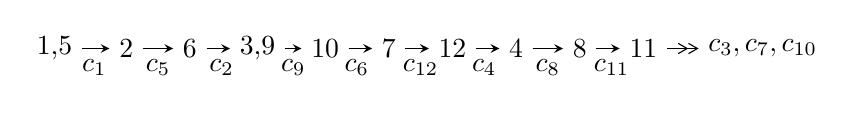
\begin{tikzpicture}[x=23pt, y=7pt]
	% node
	\node (A0) at (-1/8, 0) {1,5};
	\node (A1) at (1, 0) {2};
	\node (A2) at (2, 0) {6};
	\node (A3) at (49/16, 0) {3,9};
	\node (A4) at (33/8, 0) {10};
	\node (A5) at (41/8, 0) {7};
	\node (A6) at (49/8, 0) {12};
	\node (A7) at (57/8, 0) {4};
	\node (A8) at (65/8, 0) {8};
	\node (A9) at (73/8, 0) {11};
	\node (C1) at (1/2, -1) {$c_{1}$};
	\node (C2) at (3/2, -1) {$c_{5}$};
	\node (C3) at (5/2, -1) {$c_{2}$};
	\node (C4) at (29/8, -1) {$c_{9}$};
	\node (C5) at (37/8, -1) {$c_{6}$};
	\node (C6) at (45/8, -1) {$c_{12}$};
	\node (C7) at (53/8, -1) {$c_{4}$};
	\node (C8) at (61/8, -1) {$c_{8}$};
	\node (C9) at (69/8, -1) {$c_{11}$};
	\node (A10) at (11, 0) {$c_{3},c_{7},c_{10}$};

	% edge
	\draw[->,>=stealth]	
	(A0) edge (A1) (A1) edge (A2) (A2) edge (A3) (A3) edge (A4) (A4) edge (A5) (A5) edge (A6) (A6) edge (A7) (A7) edge (A8) (A8) edge (A9) ;
	\draw[->>,>={angle 60}]	
	(A9) edge (A10);
\end{tikzpicture} \\ 

\end{tabular} \\

\footnotetext{
The image of knot diagram is generated by the software ``\textbf{Draw programme}" developed by Andrew Bartholomew(\url{http://www.layer8.co.uk/maths/draw/index.htm\#Running-draw}), where we modified some parts for our purpose(\url{https://github.com/CATsTAILs/LinksPainter}).
}\phantom \\ \newline 
\centering \textbf{Ideals for irreducible components\footnotemark of $X_{\text{par}}$} 
 
\begin{align*}
I^u_{1}&=\langle 
4.98945\times10^{144} u^{84}-1.37087\times10^{145} u^{83}+\cdots+1.92650\times10^{144} b-2.91725\times10^{146},\\
\phantom{I^u_{1}}&\phantom{= \langle  }1.95093\times10^{145} u^{84}-5.15748\times10^{145} u^{83}+\cdots+1.40635\times10^{146} a-2.25735\times10^{147},\\
\phantom{I^u_{1}}&\phantom{= \langle  }u^{85}-4 u^{84}+\cdots+788 u+73\rangle \\
I^u_{2}&=\langle 
-5 u^{18}+13 u^{17}+\cdots+b-4,\;- u^{17}+2 u^{16}+\cdots+a-7 u,\;u^{19}- u^{18}+\cdots+4 u+1\rangle \\
I^u_{3}&=\langle 
b-1,\;- u^5+2 u^4+2 u^3-4 u^2+a- u+2,\;u^6- u^5-4 u^4+2 u^3+4 u^2+1\rangle \\
I^u_{4}&=\langle 
b-1,\;a,\;u-1\rangle \\
\\
\end{align*}
\raggedright * 4 irreducible components of $\dim_{\mathbb{C}}=0$, with total 111 representations.\\
\footnotetext{All coefficients of polynomials are rational numbers. But the coefficients are sometimes approximated in decimal forms when there is not enough margin.}
\newpage
\renewcommand{\arraystretch}{1}
\centering \section*{I. $I^u_{1}= \langle 4.99\times10^{144} u^{84}-1.37\times10^{145} u^{83}+\cdots+1.93\times10^{144} b-2.92\times10^{146},\;1.95\times10^{145} u^{84}-5.16\times10^{145} u^{83}+\cdots+1.41\times10^{146} a-2.26\times10^{147},\;u^{85}-4 u^{84}+\cdots+788 u+73 \rangle$}
\flushleft \textbf{(i) Arc colorings}\\
\begin{tabular}{m{7pt} m{180pt} m{7pt} m{180pt} }
\flushright $a_{1}=$&$\begin{pmatrix}1\\0\end{pmatrix}$ \\
\flushright $a_{5}=$&$\begin{pmatrix}0\\u\end{pmatrix}$ \\
\flushright $a_{2}=$&$\begin{pmatrix}1\\u^2\end{pmatrix}$ \\
\flushright $a_{6}=$&$\begin{pmatrix}- u\\- u^3+u\end{pmatrix}$ \\
\flushright $a_{3}=$&$\begin{pmatrix}- u^2+1\\- u^4+2 u^2\end{pmatrix}$ \\
\flushright $a_{9}=$&$\begin{pmatrix}-0.138723 u^{84}+0.366728 u^{83}+\cdots+130.193 u+16.0512\\-2.58990 u^{84}+7.11584 u^{83}+\cdots+1749.52 u+151.427\end{pmatrix}$ \\
\flushright $a_{10}=$&$\begin{pmatrix}-2.72862 u^{84}+7.48257 u^{83}+\cdots+1879.71 u+167.478\\-2.58990 u^{84}+7.11584 u^{83}+\cdots+1749.52 u+151.427\end{pmatrix}$ \\
\flushright $a_{7}=$&$\begin{pmatrix}2.92578 u^{84}-8.13708 u^{83}+\cdots-2024.72 u-177.767\\2.31664 u^{84}-6.47988 u^{83}+\cdots-1619.00 u-139.768\end{pmatrix}$ \\
\flushright $a_{12}=$&$\begin{pmatrix}0.385598 u^{84}-1.10673 u^{83}+\cdots-283.400 u-21.1009\\3.41608 u^{84}-9.58363 u^{83}+\cdots-2437.49 u-209.431\end{pmatrix}$ \\
\flushright $a_{4}=$&$\begin{pmatrix}-0.561858 u^{84}+1.48323 u^{83}+\cdots+383.494 u+32.0573\\2.75914 u^{84}-7.81915 u^{83}+\cdots-1999.66 u-171.708\end{pmatrix}$ \\
\flushright $a_{8}=$&$\begin{pmatrix}0.715497 u^{84}-2.08191 u^{83}+\cdots-538.570 u-40.4914\\1.93432 u^{84}-5.25535 u^{83}+\cdots-1247.86 u-107.161\end{pmatrix}$ \\
\flushright $a_{11}=$&$\begin{pmatrix}1.00130 u^{84}-2.85966 u^{83}+\cdots-737.962 u-59.9423\\1.84070 u^{84}-5.11536 u^{83}+\cdots-1289.48 u-110.827\end{pmatrix}$\\&\end{tabular}
\flushleft \textbf{(ii) Obstruction class $= -1$}\\~\\
\flushleft \textbf{(iii) Cusp Shapes $= 6.89483 u^{84}-19.7102 u^{83}+\cdots-4933.58 u-411.467$}\\~\\
\newpage\renewcommand{\arraystretch}{1}
\flushleft \textbf{(iv) u-Polynomials at the component}\newline \\
\begin{tabular}{m{50pt}|m{274pt}}
Crossings & \hspace{64pt}u-Polynomials at each crossing \\
\hline $$\begin{aligned}c_{1},c_{2},c_{5}\end{aligned}$$&$\begin{aligned}
&u^{85}+4 u^{84}+\cdots+788 u-73
\end{aligned}$\\
\hline $$\begin{aligned}c_{3},c_{8}\end{aligned}$$&$\begin{aligned}
&u^{85}+2 u^{84}+\cdots-13 u-1
\end{aligned}$\\
\hline $$\begin{aligned}c_{4}\end{aligned}$$&$\begin{aligned}
&u^{85}-2 u^{84}+\cdots-10671 u-1901
\end{aligned}$\\
\hline $$\begin{aligned}c_{6},c_{7},c_{10}\end{aligned}$$&$\begin{aligned}
&u^{85}-3 u^{84}+\cdots+10 u+1
\end{aligned}$\\
\hline $$\begin{aligned}c_{9},c_{12}\end{aligned}$$&$\begin{aligned}
&u^{85}+9 u^{84}+\cdots-956 u-536
\end{aligned}$\\
\hline $$\begin{aligned}c_{11}\end{aligned}$$&$\begin{aligned}
&u^{85}+6 u^{84}+\cdots-675913 u+208517
\end{aligned}$\\
\hline
\end{tabular}\\~\\
\newpage\renewcommand{\arraystretch}{1}
\flushleft \textbf{(v) Riley Polynomials at the component}\newline \\
\begin{tabular}{m{50pt}|m{274pt}}
Crossings & \hspace{64pt}Riley Polynomials at each crossing \\
\hline $$\begin{aligned}c_{1},c_{2},c_{5}\end{aligned}$$&$\begin{aligned}
&y^{85}-80 y^{84}+\cdots+416398 y-5329
\end{aligned}$\\
\hline $$\begin{aligned}c_{3},c_{8}\end{aligned}$$&$\begin{aligned}
&y^{85}-72 y^{84}+\cdots-3 y-1
\end{aligned}$\\
\hline $$\begin{aligned}c_{4}\end{aligned}$$&$\begin{aligned}
&y^{85}+16 y^{84}+\cdots-16272219 y-3613801
\end{aligned}$\\
\hline $$\begin{aligned}c_{6},c_{7},c_{10}\end{aligned}$$&$\begin{aligned}
&y^{85}-93 y^{84}+\cdots+246 y-1
\end{aligned}$\\
\hline $$\begin{aligned}c_{9},c_{12}\end{aligned}$$&$\begin{aligned}
&y^{85}-63 y^{84}+\cdots-14389936 y-287296
\end{aligned}$\\
\hline $$\begin{aligned}c_{11}\end{aligned}$$&$\begin{aligned}
&y^{85}+36 y^{84}+\cdots+2472814918725 y-43479339289
\end{aligned}$\\
\hline
\end{tabular}\\~\\
\newpage\flushleft \textbf{(vi) Complex Volumes and Cusp Shapes}
$$\begin{array}{c|c|c}  
\text{Solutions to }I^u_{1}& \I (\text{vol} + \sqrt{-1}CS) & \text{Cusp shape}\\
 \hline 
\begin{aligned}
u &= -0.624130 + 0.677501 I \\
a &= \phantom{-}1.27325 - 0.82874 I \\
b &= -1.172910 + 0.299627 I\end{aligned}
 & \phantom{-}5.48537 - 3.36947 I & \phantom{-0.000000 } 0 \\ \hline\begin{aligned}
u &= -0.624130 - 0.677501 I \\
a &= \phantom{-}1.27325 + 0.82874 I \\
b &= -1.172910 - 0.299627 I\end{aligned}
 & \phantom{-}5.48537 + 3.36947 I & \phantom{-0.000000 } 0 \\ \hline\begin{aligned}
u &= -0.409379 + 1.002590 I \\
a &= -1.68599 + 0.21190 I \\
b &= \phantom{-}1.40263 + 0.44403 I\end{aligned}
 & \phantom{-}13.5552 + 11.4881 I & \phantom{-0.000000 } 0 \\ \hline\begin{aligned}
u &= -0.409379 - 1.002590 I \\
a &= -1.68599 - 0.21190 I \\
b &= \phantom{-}1.40263 - 0.44403 I\end{aligned}
 & \phantom{-}13.5552 - 11.4881 I & \phantom{-0.000000 } 0 \\ \hline\begin{aligned}
u &= \phantom{-}1.12445\phantom{ +0.000000I} \\
a &= \phantom{-}1.58307\phantom{ +0.000000I} \\
b &= -1.67518\phantom{ +0.000000I}\end{aligned}
 & \phantom{-}11.2991\phantom{ +0.000000I} & \phantom{-0.000000 } 0 \\ \hline\begin{aligned}
u &= \phantom{-}0.301457 + 0.815530 I \\
a &= \phantom{-}1.80925 + 0.18621 I \\
b &= -1.029340 + 0.250303 I\end{aligned}
 & \phantom{-}1.17315 - 3.20365 I & \phantom{-0.000000 } 0 \\ \hline\begin{aligned}
u &= \phantom{-}0.301457 - 0.815530 I \\
a &= \phantom{-}1.80925 - 0.18621 I \\
b &= -1.029340 - 0.250303 I\end{aligned}
 & \phantom{-}1.17315 + 3.20365 I & \phantom{-0.000000 } 0 \\ \hline\begin{aligned}
u &= -1.149180 + 0.081342 I \\
a &= \phantom{-}1.03377 + 1.54266 I \\
b &= -0.850018 - 0.005837 I\end{aligned}
 & \phantom{-}6.06553 + 5.53345 I & \phantom{-0.000000 } 0 \\ \hline\begin{aligned}
u &= -1.149180 - 0.081342 I \\
a &= \phantom{-}1.03377 - 1.54266 I \\
b &= -0.850018 + 0.005837 I\end{aligned}
 & \phantom{-}6.06553 - 5.53345 I & \phantom{-0.000000 } 0 \\ \hline\begin{aligned}
u &= \phantom{-}1.164800 + 0.089757 I \\
a &= \phantom{-}0.52166 - 1.45972 I \\
b &= -0.799484 - 0.495047 I\end{aligned}
 & \phantom{-}1.60587 - 0.73292 I & \phantom{-0.000000 } 0\\
 \hline 
 \end{array}$$\newpage$$\begin{array}{c|c|c}  
\text{Solutions to }I^u_{1}& \I (\text{vol} + \sqrt{-1}CS) & \text{Cusp shape}\\
 \hline 
\begin{aligned}
u &= \phantom{-}1.164800 - 0.089757 I \\
a &= \phantom{-}0.52166 + 1.45972 I \\
b &= -0.799484 + 0.495047 I\end{aligned}
 & \phantom{-}1.60587 + 0.73292 I & \phantom{-0.000000 } 0 \\ \hline\begin{aligned}
u &= -1.16926\phantom{ +0.000000I} \\
a &= \phantom{-}0.845667\phantom{ +0.000000I} \\
b &= -1.78576\phantom{ +0.000000I}\end{aligned}
 & \phantom{-}6.73023\phantom{ +0.000000I} & \phantom{-0.000000 } 0 \\ \hline\begin{aligned}
u &= \phantom{-}0.192937 + 1.154220 I \\
a &= -1.44238 - 0.07519 I \\
b &= \phantom{-}1.087730 - 0.364012 I\end{aligned}
 & \phantom{-}6.71901 - 5.49463 I & \phantom{-0.000000 } 0 \\ \hline\begin{aligned}
u &= \phantom{-}0.192937 - 1.154220 I \\
a &= -1.44238 + 0.07519 I \\
b &= \phantom{-}1.087730 + 0.364012 I\end{aligned}
 & \phantom{-}6.71901 + 5.49463 I & \phantom{-0.000000 } 0 \\ \hline\begin{aligned}
u &= -0.360617 + 0.745031 I \\
a &= \phantom{-}2.20948 - 0.41944 I \\
b &= -1.300800 - 0.407023 I\end{aligned}
 & \phantom{-}6.28975 + 7.97133 I & \phantom{-}7.38430 - 8.02100 I \\ \hline\begin{aligned}
u &= -0.360617 - 0.745031 I \\
a &= \phantom{-}2.20948 + 0.41944 I \\
b &= -1.300800 + 0.407023 I\end{aligned}
 & \phantom{-}6.28975 - 7.97133 I & \phantom{-}7.38430 + 8.02100 I \\ \hline\begin{aligned}
u &= -1.198080 + 0.082837 I \\
a &= \phantom{-}0.214684 + 1.075630 I \\
b &= -1.12156 + 0.98848 I\end{aligned}
 & \phantom{-}5.68630 - 4.05640 I & \phantom{-0.000000 } 0 \\ \hline\begin{aligned}
u &= -1.198080 - 0.082837 I \\
a &= \phantom{-}0.214684 - 1.075630 I \\
b &= -1.12156 - 0.98848 I\end{aligned}
 & \phantom{-}5.68630 + 4.05640 I & \phantom{-0.000000 } 0 \\ \hline\begin{aligned}
u &= \phantom{-}1.20730\phantom{ +0.000000I} \\
a &= \phantom{-}0.288478\phantom{ +0.000000I} \\
b &= -2.30164\phantom{ +0.000000I}\end{aligned}
 & \phantom{-}10.5815\phantom{ +0.000000I} & \phantom{-0.000000 } 0 \\ \hline\begin{aligned}
u &= \phantom{-}0.345771 + 0.669877 I \\
a &= \phantom{-}1.28934 + 1.71832 I \\
b &= -1.339630 - 0.095594 I\end{aligned}
 & \phantom{-}12.65180 - 2.38566 I & \phantom{-}11.28357 + 3.13973 I\\
 \hline 
 \end{array}$$\newpage$$\begin{array}{c|c|c}  
\text{Solutions to }I^u_{1}& \I (\text{vol} + \sqrt{-1}CS) & \text{Cusp shape}\\
 \hline 
\begin{aligned}
u &= \phantom{-}0.345771 - 0.669877 I \\
a &= \phantom{-}1.28934 - 1.71832 I \\
b &= -1.339630 + 0.095594 I\end{aligned}
 & \phantom{-}12.65180 + 2.38566 I & \phantom{-}11.28357 - 3.13973 I \\ \hline\begin{aligned}
u &= -0.369159 + 0.631904 I \\
a &= \phantom{-}1.18727 - 0.96387 I \\
b &= -1.314670 - 0.246770 I\end{aligned}
 & \phantom{-}8.21278 + 1.87881 I & \phantom{-}10.83009 - 0.57094 I \\ \hline\begin{aligned}
u &= -0.369159 - 0.631904 I \\
a &= \phantom{-}1.18727 + 0.96387 I \\
b &= -1.314670 + 0.246770 I\end{aligned}
 & \phantom{-}8.21278 - 1.87881 I & \phantom{-}10.83009 + 0.57094 I \\ \hline\begin{aligned}
u &= \phantom{-}0.395662 + 0.581191 I \\
a &= \phantom{-}1.48354 + 0.44038 I \\
b &= -1.60987 + 0.54830 I\end{aligned}
 & \phantom{-}12.29370 - 1.36558 I & \phantom{-}11.35480 + 4.41215 I \\ \hline\begin{aligned}
u &= \phantom{-}0.395662 - 0.581191 I \\
a &= \phantom{-}1.48354 - 0.44038 I \\
b &= -1.60987 - 0.54830 I\end{aligned}
 & \phantom{-}12.29370 + 1.36558 I & \phantom{-}11.35480 - 4.41215 I \\ \hline\begin{aligned}
u &= \phantom{-}0.252051 + 0.653041 I \\
a &= -0.757441 + 0.041642 I \\
b &= \phantom{-}0.067707 + 0.675510 I\end{aligned}
 & \phantom{-}3.87059 - 1.76215 I & \phantom{-}3.74742 + 3.64728 I \\ \hline\begin{aligned}
u &= \phantom{-}0.252051 - 0.653041 I \\
a &= -0.757441 - 0.041642 I \\
b &= \phantom{-}0.067707 - 0.675510 I\end{aligned}
 & \phantom{-}3.87059 + 1.76215 I & \phantom{-}3.74742 - 3.64728 I \\ \hline\begin{aligned}
u &= -0.323184 + 0.612844 I \\
a &= -1.34257 - 1.28161 I \\
b &= \phantom{-}0.014273 + 0.180616 I\end{aligned}
 & \phantom{-}8.16304 - 3.16907 I & \phantom{-}8.19689 - 1.41717 I \\ \hline\begin{aligned}
u &= -0.323184 - 0.612844 I \\
a &= -1.34257 + 1.28161 I \\
b &= \phantom{-}0.014273 - 0.180616 I\end{aligned}
 & \phantom{-}8.16304 + 3.16907 I & \phantom{-}8.19689 + 1.41717 I \\ \hline\begin{aligned}
u &= -0.910397 + 0.940971 I \\
a &= -0.942683 + 0.660065 I \\
b &= \phantom{-}1.261770 - 0.234880 I\end{aligned}
 & \phantom{-}12.19520 - 5.09209 I & \phantom{-0.000000 } 0\\
 \hline 
 \end{array}$$\newpage$$\begin{array}{c|c|c}  
\text{Solutions to }I^u_{1}& \I (\text{vol} + \sqrt{-1}CS) & \text{Cusp shape}\\
 \hline 
\begin{aligned}
u &= -0.910397 - 0.940971 I \\
a &= -0.942683 - 0.660065 I \\
b &= \phantom{-}1.261770 + 0.234880 I\end{aligned}
 & \phantom{-}12.19520 + 5.09209 I & \phantom{-0.000000 } 0 \\ \hline\begin{aligned}
u &= \phantom{-}1.31174\phantom{ +0.000000I} \\
a &= -0.512904\phantom{ +0.000000I} \\
b &= \phantom{-}1.29127\phantom{ +0.000000I}\end{aligned}
 & \phantom{-}1.49689\phantom{ +0.000000I} & \phantom{-0.000000 } 0 \\ \hline\begin{aligned}
u &= \phantom{-}1.310290 + 0.142010 I \\
a &= -0.460124 - 1.144650 I \\
b &= \phantom{-}0.950477 - 0.477408 I\end{aligned}
 & -2.39006 - 2.09627 I & \phantom{-0.000000 } 0 \\ \hline\begin{aligned}
u &= \phantom{-}1.310290 - 0.142010 I \\
a &= -0.460124 + 1.144650 I \\
b &= \phantom{-}0.950477 + 0.477408 I\end{aligned}
 & -2.39006 + 2.09627 I & \phantom{-0.000000 } 0 \\ \hline\begin{aligned}
u &= -1.315430 + 0.140434 I \\
a &= -0.389970 + 0.923304 I \\
b &= \phantom{-}1.30169 + 0.95849 I\end{aligned}
 & \phantom{-}1.18769 + 4.19202 I & \phantom{-0.000000 } 0 \\ \hline\begin{aligned}
u &= -1.315430 - 0.140434 I \\
a &= -0.389970 - 0.923304 I \\
b &= \phantom{-}1.30169 - 0.95849 I\end{aligned}
 & \phantom{-}1.18769 - 4.19202 I & \phantom{-0.000000 } 0 \\ \hline\begin{aligned}
u &= \phantom{-}1.333230 + 0.195789 I \\
a &= -1.47363 - 1.02765 I \\
b &= \phantom{-}1.40909 - 0.37140 I\end{aligned}
 & \phantom{-}1.00589 - 5.05324 I & \phantom{-0.000000 } 0 \\ \hline\begin{aligned}
u &= \phantom{-}1.333230 - 0.195789 I \\
a &= -1.47363 + 1.02765 I \\
b &= \phantom{-}1.40909 + 0.37140 I\end{aligned}
 & \phantom{-}1.00589 + 5.05324 I & \phantom{-0.000000 } 0 \\ \hline\begin{aligned}
u &= -1.353310 + 0.168736 I \\
a &= -1.135850 + 0.671511 I \\
b &= \phantom{-}1.275170 + 0.382326 I\end{aligned}
 & -2.89149 + 2.20435 I & \phantom{-0.000000 } 0 \\ \hline\begin{aligned}
u &= -1.353310 - 0.168736 I \\
a &= -1.135850 - 0.671511 I \\
b &= \phantom{-}1.275170 - 0.382326 I\end{aligned}
 & -2.89149 - 2.20435 I & \phantom{-0.000000 } 0\\
 \hline 
 \end{array}$$\newpage$$\begin{array}{c|c|c}  
\text{Solutions to }I^u_{1}& \I (\text{vol} + \sqrt{-1}CS) & \text{Cusp shape}\\
 \hline 
\begin{aligned}
u &= -0.260065 + 0.576274 I \\
a &= -0.138226 + 0.392642 I \\
b &= -0.337232 - 1.153370 I\end{aligned}
 & \phantom{-}8.20231 + 6.17948 I & \phantom{-}8.20026 - 7.53712 I \\ \hline\begin{aligned}
u &= -0.260065 - 0.576274 I \\
a &= -0.138226 - 0.392642 I \\
b &= -0.337232 + 1.153370 I\end{aligned}
 & \phantom{-}8.20231 - 6.17948 I & \phantom{-}8.20026 + 7.53712 I \\ \hline\begin{aligned}
u &= -0.400208 + 0.472091 I \\
a &= -0.384579 - 0.514091 I \\
b &= \phantom{-}0.143077 + 0.872180 I\end{aligned}
 & \phantom{-}1.90136 + 3.46440 I & \phantom{-}4.11990 - 8.09520 I \\ \hline\begin{aligned}
u &= -0.400208 - 0.472091 I \\
a &= -0.384579 + 0.514091 I \\
b &= \phantom{-}0.143077 - 0.872180 I\end{aligned}
 & \phantom{-}1.90136 - 3.46440 I & \phantom{-}4.11990 + 8.09520 I \\ \hline\begin{aligned}
u &= \phantom{-}0.524761 + 0.282395 I \\
a &= \phantom{-}0.431371 + 0.231054 I \\
b &= -0.168767 - 0.371547 I\end{aligned}
 & -1.053160 - 0.578747 I & -6.16527 + 2.76686 I \\ \hline\begin{aligned}
u &= \phantom{-}0.524761 - 0.282395 I \\
a &= \phantom{-}0.431371 - 0.231054 I \\
b &= -0.168767 + 0.371547 I\end{aligned}
 & -1.053160 + 0.578747 I & -6.16527 - 2.76686 I \\ \hline\begin{aligned}
u &= \phantom{-}1.347350 + 0.409713 I \\
a &= \phantom{-}0.949410 + 0.561746 I \\
b &= -0.935806 + 0.242242 I\end{aligned}
 & -1.77639 - 1.77523 I & \phantom{-0.000000 } 0 \\ \hline\begin{aligned}
u &= \phantom{-}1.347350 - 0.409713 I \\
a &= \phantom{-}0.949410 - 0.561746 I \\
b &= -0.935806 - 0.242242 I\end{aligned}
 & -1.77639 + 1.77523 I & \phantom{-0.000000 } 0 \\ \hline\begin{aligned}
u &= -1.387010 + 0.261595 I \\
a &= \phantom{-}0.036469 - 0.262545 I \\
b &= \phantom{-}0.347098 - 1.080660 I\end{aligned}
 & -1.31353 + 5.12324 I & \phantom{-0.000000 } 0 \\ \hline\begin{aligned}
u &= -1.387010 - 0.261595 I \\
a &= \phantom{-}0.036469 + 0.262545 I \\
b &= \phantom{-}0.347098 + 1.080660 I\end{aligned}
 & -1.31353 - 5.12324 I & \phantom{-0.000000 } 0\\
 \hline 
 \end{array}$$\newpage$$\begin{array}{c|c|c}  
\text{Solutions to }I^u_{1}& \I (\text{vol} + \sqrt{-1}CS) & \text{Cusp shape}\\
 \hline 
\begin{aligned}
u &= \phantom{-}1.40272 + 0.23901 I \\
a &= \phantom{-}0.252195 + 0.345108 I \\
b &= \phantom{-}0.01364 + 1.55109 I\end{aligned}
 & \phantom{-}2.87646 - 9.22644 I & \phantom{-0.000000 } 0 \\ \hline\begin{aligned}
u &= \phantom{-}1.40272 - 0.23901 I \\
a &= \phantom{-}0.252195 - 0.345108 I \\
b &= \phantom{-}0.01364 - 1.55109 I\end{aligned}
 & \phantom{-}2.87646 + 9.22644 I & \phantom{-0.000000 } 0 \\ \hline\begin{aligned}
u &= -0.375540 + 0.431749 I \\
a &= \phantom{-}1.146050 + 0.602010 I \\
b &= \phantom{-}0.047218 - 0.523660 I\end{aligned}
 & \phantom{-}1.96018 - 0.39806 I & \phantom{-}4.48273 - 0.63616 I \\ \hline\begin{aligned}
u &= -0.375540 - 0.431749 I \\
a &= \phantom{-}1.146050 - 0.602010 I \\
b &= \phantom{-}0.047218 + 0.523660 I\end{aligned}
 & \phantom{-}1.96018 + 0.39806 I & \phantom{-}4.48273 + 0.63616 I \\ \hline\begin{aligned}
u &= \phantom{-}1.38602 + 0.37040 I \\
a &= -0.400754 + 0.063344 I \\
b &= \phantom{-}0.711046 + 0.385814 I\end{aligned}
 & \phantom{-}2.31278 - 0.56245 I & \phantom{-0.000000 } 0 \\ \hline\begin{aligned}
u &= \phantom{-}1.38602 - 0.37040 I \\
a &= -0.400754 - 0.063344 I \\
b &= \phantom{-}0.711046 - 0.385814 I\end{aligned}
 & \phantom{-}2.31278 + 0.56245 I & \phantom{-0.000000 } 0 \\ \hline\begin{aligned}
u &= \phantom{-}1.43721 + 0.03949 I \\
a &= \phantom{-}0.501581 + 0.307898 I \\
b &= -0.100119 + 0.665742 I\end{aligned}
 & -3.84830 - 1.03714 I & \phantom{-0.000000 } 0 \\ \hline\begin{aligned}
u &= \phantom{-}1.43721 - 0.03949 I \\
a &= \phantom{-}0.501581 - 0.307898 I \\
b &= -0.100119 - 0.665742 I\end{aligned}
 & -3.84830 + 1.03714 I & \phantom{-0.000000 } 0 \\ \hline\begin{aligned}
u &= \phantom{-}1.43195 + 0.14709 I \\
a &= -0.329587 - 0.361408 I \\
b &= \phantom{-}0.027993 - 1.196330 I\end{aligned}
 & -3.98333 - 5.67696 I & \phantom{-0.000000 } 0 \\ \hline\begin{aligned}
u &= \phantom{-}1.43195 - 0.14709 I \\
a &= -0.329587 + 0.361408 I \\
b &= \phantom{-}0.027993 + 1.196330 I\end{aligned}
 & -3.98333 + 5.67696 I & \phantom{-0.000000 } 0\\
 \hline 
 \end{array}$$\newpage$$\begin{array}{c|c|c}  
\text{Solutions to }I^u_{1}& \I (\text{vol} + \sqrt{-1}CS) & \text{Cusp shape}\\
 \hline 
\begin{aligned}
u &= -1.42782 + 0.30450 I \\
a &= \phantom{-}1.029350 - 0.806960 I \\
b &= -1.203740 - 0.522812 I\end{aligned}
 & -4.35157 + 7.18408 I & \phantom{-0.000000 } 0 \\ \hline\begin{aligned}
u &= -1.42782 - 0.30450 I \\
a &= \phantom{-}1.029350 + 0.806960 I \\
b &= -1.203740 + 0.522812 I\end{aligned}
 & -4.35157 - 7.18408 I & \phantom{-0.000000 } 0 \\ \hline\begin{aligned}
u &= -1.45967 + 0.09531 I \\
a &= -0.022628 + 0.249071 I \\
b &= -0.182505 + 0.900172 I\end{aligned}
 & -7.48171 + 2.02794 I & \phantom{-0.000000 } 0 \\ \hline\begin{aligned}
u &= -1.45967 - 0.09531 I \\
a &= -0.022628 - 0.249071 I \\
b &= -0.182505 - 0.900172 I\end{aligned}
 & -7.48171 - 2.02794 I & \phantom{-0.000000 } 0 \\ \hline\begin{aligned}
u &= -0.058099 + 0.526758 I \\
a &= -3.74437 - 0.86928 I \\
b &= \phantom{-}1.226770 + 0.248698 I\end{aligned}
 & \phantom{-}5.43767 + 2.43332 I & \phantom{-}12.27217 - 3.91915 I \\ \hline\begin{aligned}
u &= -0.058099 - 0.526758 I \\
a &= -3.74437 + 0.86928 I \\
b &= \phantom{-}1.226770 - 0.248698 I\end{aligned}
 & \phantom{-}5.43767 - 2.43332 I & \phantom{-}12.27217 + 3.91915 I \\ \hline\begin{aligned}
u &= -1.44411 + 0.28089 I \\
a &= \phantom{-}0.124422 - 1.264770 I \\
b &= -1.062120 - 0.060649 I\end{aligned}
 & \phantom{-}6.90944 + 5.91266 I & \phantom{-0.000000 } 0 \\ \hline\begin{aligned}
u &= -1.44411 - 0.28089 I \\
a &= \phantom{-}0.124422 + 1.264770 I \\
b &= -1.062120 + 0.060649 I\end{aligned}
 & \phantom{-}6.90944 - 5.91266 I & \phantom{-0.000000 } 0 \\ \hline\begin{aligned}
u &= \phantom{-}1.44817 + 0.26550 I \\
a &= \phantom{-}0.250173 + 0.920078 I \\
b &= -1.070750 + 0.553524 I\end{aligned}
 & \phantom{-}2.37812 - 5.23342 I & \phantom{-0.000000 } 0 \\ \hline\begin{aligned}
u &= \phantom{-}1.44817 - 0.26550 I \\
a &= \phantom{-}0.250173 - 0.920078 I \\
b &= -1.070750 - 0.553524 I\end{aligned}
 & \phantom{-}2.37812 + 5.23342 I & \phantom{-0.000000 } 0\\
 \hline 
 \end{array}$$\newpage$$\begin{array}{c|c|c}  
\text{Solutions to }I^u_{1}& \I (\text{vol} + \sqrt{-1}CS) & \text{Cusp shape}\\
 \hline 
\begin{aligned}
u &= \phantom{-}1.44320 + 0.29402 I \\
a &= \phantom{-}1.07173 + 1.00849 I \\
b &= -1.40089 + 0.55110 I\end{aligned}
 & \phantom{-}0.53532 - 11.75990 I & \phantom{-0.000000 } 0 \\ \hline\begin{aligned}
u &= \phantom{-}1.44320 - 0.29402 I \\
a &= \phantom{-}1.07173 - 1.00849 I \\
b &= -1.40089 - 0.55110 I\end{aligned}
 & \phantom{-}0.53532 + 11.75990 I & \phantom{-0.000000 } 0 \\ \hline\begin{aligned}
u &= -1.45461 + 0.24376 I \\
a &= \phantom{-}0.389692 - 0.802347 I \\
b &= -1.41742 - 1.00679 I\end{aligned}
 & \phantom{-}6.34695 + 4.48091 I & \phantom{-0.000000 } 0 \\ \hline\begin{aligned}
u &= -1.45461 - 0.24376 I \\
a &= \phantom{-}0.389692 + 0.802347 I \\
b &= -1.41742 + 1.00679 I\end{aligned}
 & \phantom{-}6.34695 - 4.48091 I & \phantom{-0.000000 } 0 \\ \hline\begin{aligned}
u &= \phantom{-}1.28916 + 0.74858 I \\
a &= -1.223760 - 0.579291 I \\
b &= \phantom{-}0.863011 - 0.274783 I\end{aligned}
 & \phantom{-}2.61452 - 3.50027 I & \phantom{-0.000000 } 0 \\ \hline\begin{aligned}
u &= \phantom{-}1.28916 - 0.74858 I \\
a &= -1.223760 + 0.579291 I \\
b &= \phantom{-}0.863011 + 0.274783 I\end{aligned}
 & \phantom{-}2.61452 + 3.50027 I & \phantom{-0.000000 } 0 \\ \hline\begin{aligned}
u &= -0.000669 + 0.479428 I \\
a &= -2.21076 + 0.10853 I \\
b &= \phantom{-}1.33078 - 0.51074 I\end{aligned}
 & \phantom{-}5.30975 - 2.02687 I & \phantom{-}14.9012 + 3.2094 I \\ \hline\begin{aligned}
u &= -0.000669 - 0.479428 I \\
a &= -2.21076 - 0.10853 I \\
b &= \phantom{-}1.33078 + 0.51074 I\end{aligned}
 & \phantom{-}5.30975 + 2.02687 I & \phantom{-}14.9012 - 3.2094 I \\ \hline\begin{aligned}
u &= -1.45774 + 0.44477 I \\
a &= -0.986710 + 0.825536 I \\
b &= \phantom{-}1.192490 + 0.605367 I\end{aligned}
 & \phantom{-}1.39761 + 11.05220 I & \phantom{-0.000000 } 0 \\ \hline\begin{aligned}
u &= -1.45774 - 0.44477 I \\
a &= -0.986710 - 0.825536 I \\
b &= \phantom{-}1.192490 - 0.605367 I\end{aligned}
 & \phantom{-}1.39761 - 11.05220 I & \phantom{-0.000000 } 0\\
 \hline 
 \end{array}$$\newpage$$\begin{array}{c|c|c}  
\text{Solutions to }I^u_{1}& \I (\text{vol} + \sqrt{-1}CS) & \text{Cusp shape}\\
 \hline 
\begin{aligned}
u &= \phantom{-}1.50394 + 0.39283 I \\
a &= -0.947921 - 0.892330 I \\
b &= \phantom{-}1.44979 - 0.64447 I\end{aligned}
 & \phantom{-}7.4665 - 16.5073 I & \phantom{-0.000000 } 0 \\ \hline\begin{aligned}
u &= \phantom{-}1.50394 - 0.39283 I \\
a &= -0.947921 + 0.892330 I \\
b &= \phantom{-}1.44979 + 0.64447 I\end{aligned}
 & \phantom{-}7.4665 + 16.5073 I & \phantom{-0.000000 } 0 \\ \hline\begin{aligned}
u &= -1.63342\phantom{ +0.000000I} \\
a &= \phantom{-}0.200193\phantom{ +0.000000I} \\
b &= \phantom{-}0.420791\phantom{ +0.000000I}\end{aligned}
 & -7.19573\phantom{ +0.000000I} & \phantom{-0.000000 } 0 \\ \hline\begin{aligned}
u &= \phantom{-}1.72107\phantom{ +0.000000I} \\
a &= \phantom{-}0.418682\phantom{ +0.000000I} \\
b &= -0.809091\phantom{ +0.000000I}\end{aligned}
 & -3.01365\phantom{ +0.000000I} & \phantom{-0.000000 } 0 \\ \hline\begin{aligned}
u &= -0.106379\phantom{ +0.000000I} \\
a &= \phantom{-}5.09497\phantom{ +0.000000I} \\
b &= \phantom{-}0.447981\phantom{ +0.000000I}\end{aligned}
 & \phantom{-}0.879411\phantom{ +0.000000I} & \phantom{-}12.9870\phantom{ +0.000000I}\\
 \hline 
 \end{array}$$\newpage\newpage\renewcommand{\arraystretch}{1}
\centering \section*{II. $I^u_{2}= \langle -5 u^{18}+13 u^{17}+\cdots+b-4,\;- u^{17}+2 u^{16}+\cdots+a-7 u,\;u^{19}- u^{18}+\cdots+4 u+1 \rangle$}
\flushleft \textbf{(i) Arc colorings}\\
\begin{tabular}{m{7pt} m{180pt} m{7pt} m{180pt} }
\flushright $a_{1}=$&$\begin{pmatrix}1\\0\end{pmatrix}$ \\
\flushright $a_{5}=$&$\begin{pmatrix}0\\u\end{pmatrix}$ \\
\flushright $a_{2}=$&$\begin{pmatrix}1\\u^2\end{pmatrix}$ \\
\flushright $a_{6}=$&$\begin{pmatrix}- u\\- u^3+u\end{pmatrix}$ \\
\flushright $a_{3}=$&$\begin{pmatrix}- u^2+1\\- u^4+2 u^2\end{pmatrix}$ \\
\flushright $a_{9}=$&$\begin{pmatrix}u^{17}-2 u^{16}+\cdots-4 u^2+7 u\\5 u^{18}-13 u^{17}+\cdots+12 u+4\end{pmatrix}$ \\
\flushright $a_{10}=$&$\begin{pmatrix}5 u^{18}-12 u^{17}+\cdots+19 u+4\\5 u^{18}-13 u^{17}+\cdots+12 u+4\end{pmatrix}$ \\
\flushright $a_{7}=$&$\begin{pmatrix}-2 u^{18}+4 u^{17}+\cdots-8 u-2\\3 u^{18}-7 u^{17}+\cdots+7 u^2+5 u\end{pmatrix}$ \\
\flushright $a_{12}=$&$\begin{pmatrix}3 u^{18}-5 u^{17}+\cdots+20 u+6\\-2 u^{18}+5 u^{17}+\cdots-9 u-1\end{pmatrix}$ \\
\flushright $a_{4}=$&$\begin{pmatrix}2 u^{18}-7 u^{17}+\cdots-5 u+2\\-3 u^{18}+6 u^{17}+\cdots-7 u-5\end{pmatrix}$ \\
\flushright $a_{8}=$&$\begin{pmatrix}-4 u^{18}+9 u^{17}+\cdots-14 u-1\\-4 u^{18}+9 u^{17}+\cdots-7 u-3\end{pmatrix}$ \\
\flushright $a_{11}=$&$\begin{pmatrix}3 u^{18}-5 u^{17}+\cdots+18 u+6\\- u^{18}+3 u^{17}+\cdots-3 u^2-6 u\end{pmatrix}$\\&\end{tabular}
\flushleft \textbf{(ii) Obstruction class $= 1$}\\~\\
\flushleft \textbf{(iii) Cusp Shapes $= 8 u^{18}-12 u^{17}-84 u^{16}+122 u^{15}+366 u^{14}-508 u^{13}-858 u^{12}+1087 u^{11}+1167 u^{10}-1187 u^9-913 u^8+474 u^7+369 u^6+174 u^5-43 u^4-150 u^3-15 u^2+7 u+10$}\\~\\
\newpage\renewcommand{\arraystretch}{1}
\flushleft \textbf{(iv) u-Polynomials at the component}\newline \\
\begin{tabular}{m{50pt}|m{274pt}}
Crossings & \hspace{64pt}u-Polynomials at each crossing \\
\hline $$\begin{aligned}c_{1},c_{2}\end{aligned}$$&$\begin{aligned}
&u^{19}- u^{18}+\cdots+4 u+1
\end{aligned}$\\
\hline $$\begin{aligned}c_{3}\end{aligned}$$&$\begin{aligned}
&u^{19}+u^{18}+\cdots- u-1
\end{aligned}$\\
\hline $$\begin{aligned}c_{4}\end{aligned}$$&$\begin{aligned}
&u^{19}+u^{18}+\cdots+u-1
\end{aligned}$\\
\hline $$\begin{aligned}c_{5}\end{aligned}$$&$\begin{aligned}
&u^{19}+u^{18}+\cdots+4 u-1
\end{aligned}$\\
\hline $$\begin{aligned}c_{6},c_{7}\end{aligned}$$&$\begin{aligned}
&u^{19}-2 u^{18}+\cdots+2 u-1
\end{aligned}$\\
\hline $$\begin{aligned}c_{8}\end{aligned}$$&$\begin{aligned}
&u^{19}- u^{18}+\cdots- u+1
\end{aligned}$\\
\hline $$\begin{aligned}c_{9}\end{aligned}$$&$\begin{aligned}
&u^{19}-3 u^{18}+\cdots+7 u+1
\end{aligned}$\\
\hline $$\begin{aligned}c_{10}\end{aligned}$$&$\begin{aligned}
&u^{19}+2 u^{18}+\cdots+2 u+1
\end{aligned}$\\
\hline $$\begin{aligned}c_{11}\end{aligned}$$&$\begin{aligned}
&u^{19}- u^{18}+\cdots+5 u-1
\end{aligned}$\\
\hline $$\begin{aligned}c_{12}\end{aligned}$$&$\begin{aligned}
&u^{19}+3 u^{18}+\cdots+7 u-1
\end{aligned}$\\
\hline
\end{tabular}\\~\\
\newpage\renewcommand{\arraystretch}{1}
\flushleft \textbf{(v) Riley Polynomials at the component}\newline \\
\begin{tabular}{m{50pt}|m{274pt}}
Crossings & \hspace{64pt}Riley Polynomials at each crossing \\
\hline $$\begin{aligned}c_{1},c_{2},c_{5}\end{aligned}$$&$\begin{aligned}
&y^{19}-25 y^{18}+\cdots+6 y-1
\end{aligned}$\\
\hline $$\begin{aligned}c_{3},c_{8}\end{aligned}$$&$\begin{aligned}
&y^{19}-21 y^{18}+\cdots+45 y-1
\end{aligned}$\\
\hline $$\begin{aligned}c_{4}\end{aligned}$$&$\begin{aligned}
&y^{19}+3 y^{18}+\cdots+13 y-1
\end{aligned}$\\
\hline $$\begin{aligned}c_{6},c_{7},c_{10}\end{aligned}$$&$\begin{aligned}
&y^{19}-22 y^{18}+\cdots+10 y-1
\end{aligned}$\\
\hline $$\begin{aligned}c_{9},c_{12}\end{aligned}$$&$\begin{aligned}
&y^{19}-21 y^{18}+\cdots+61 y-1
\end{aligned}$\\
\hline $$\begin{aligned}c_{11}\end{aligned}$$&$\begin{aligned}
&y^{19}+3 y^{18}+\cdots+9 y-1
\end{aligned}$\\
\hline
\end{tabular}\\~\\
\newpage\flushleft \textbf{(vi) Complex Volumes and Cusp Shapes}
$$\begin{array}{c|c|c}  
\text{Solutions to }I^u_{2}& \I (\text{vol} + \sqrt{-1}CS) & \text{Cusp shape}\\
 \hline 
\begin{aligned}
u &= \phantom{-}1.10278\phantom{ +0.000000I} \\
a &= \phantom{-}0.720093\phantom{ +0.000000I} \\
b &= -1.70355\phantom{ +0.000000I}\end{aligned}
 & \phantom{-}6.99800\phantom{ +0.000000I} & \phantom{-}17.7350\phantom{ +0.000000I} \\ \hline\begin{aligned}
u &= -1.26024\phantom{ +0.000000I} \\
a &= \phantom{-}0.906514\phantom{ +0.000000I} \\
b &= -2.09527\phantom{ +0.000000I}\end{aligned}
 & \phantom{-}9.84855\phantom{ +0.000000I} & \phantom{-}0.542410\phantom{ +0.000000I} \\ \hline\begin{aligned}
u &= \phantom{-}1.253900 + 0.227809 I \\
a &= -0.900344 - 0.843791 I \\
b &= \phantom{-}1.020270 - 0.265725 I\end{aligned}
 & -1.12863 - 1.33201 I & \phantom{-}5.39680 - 0.05843 I \\ \hline\begin{aligned}
u &= \phantom{-}1.253900 - 0.227809 I \\
a &= -0.900344 + 0.843791 I \\
b &= \phantom{-}1.020270 + 0.265725 I\end{aligned}
 & -1.12863 + 1.33201 I & \phantom{-}5.39680 + 0.05843 I \\ \hline\begin{aligned}
u &= -1.327440 + 0.099919 I \\
a &= -0.693739 + 1.130910 I \\
b &= \phantom{-}1.32837 + 0.65411 I\end{aligned}
 & \phantom{-}0.65874 + 3.18643 I & \phantom{-}2.84941 - 0.30702 I \\ \hline\begin{aligned}
u &= -1.327440 - 0.099919 I \\
a &= -0.693739 - 1.130910 I \\
b &= \phantom{-}1.32837 - 0.65411 I\end{aligned}
 & \phantom{-}0.65874 - 3.18643 I & \phantom{-}2.84941 + 0.30702 I \\ \hline\begin{aligned}
u &= -1.374240 + 0.196813 I \\
a &= -0.000109 - 1.119420 I \\
b &= -0.831567 - 0.883831 I\end{aligned}
 & \phantom{-}4.21440 + 7.04159 I & \phantom{-}4.96365 - 5.87415 I \\ \hline\begin{aligned}
u &= -1.374240 - 0.196813 I \\
a &= -0.000109 + 1.119420 I \\
b &= -0.831567 + 0.883831 I\end{aligned}
 & \phantom{-}4.21440 - 7.04159 I & \phantom{-}4.96365 + 5.87415 I \\ \hline\begin{aligned}
u &= -0.134296 + 0.586065 I \\
a &= \phantom{-}2.35029 + 0.60951 I \\
b &= -0.916608 + 0.500115 I\end{aligned}
 & \phantom{-}8.54052 - 4.44138 I & \phantom{-}11.11085 + 4.14729 I \\ \hline\begin{aligned}
u &= -0.134296 - 0.586065 I \\
a &= \phantom{-}2.35029 - 0.60951 I \\
b &= -0.916608 - 0.500115 I\end{aligned}
 & \phantom{-}8.54052 + 4.44138 I & \phantom{-}11.11085 - 4.14729 I\\
 \hline 
 \end{array}$$\newpage$$\begin{array}{c|c|c}  
\text{Solutions to }I^u_{2}& \I (\text{vol} + \sqrt{-1}CS) & \text{Cusp shape}\\
 \hline 
\begin{aligned}
u &= \phantom{-}1.35294 + 0.54742 I \\
a &= \phantom{-}0.862592 + 0.861954 I \\
b &= -0.811030 + 0.265564 I\end{aligned}
 & \phantom{-}2.63803 - 2.91120 I & \phantom{-}5.09455 - 1.50399 I \\ \hline\begin{aligned}
u &= \phantom{-}1.35294 - 0.54742 I \\
a &= \phantom{-}0.862592 - 0.861954 I \\
b &= -0.811030 - 0.265564 I\end{aligned}
 & \phantom{-}2.63803 + 2.91120 I & \phantom{-}5.09455 + 1.50399 I \\ \hline\begin{aligned}
u &= \phantom{-}0.539160\phantom{ +0.000000I} \\
a &= \phantom{-}1.08291\phantom{ +0.000000I} \\
b &= \phantom{-}0.394778\phantom{ +0.000000I}\end{aligned}
 & \phantom{-}0.237359\phantom{ +0.000000I} & -2.52210\phantom{ +0.000000I} \\ \hline\begin{aligned}
u &= -0.466068\phantom{ +0.000000I} \\
a &= -0.590861\phantom{ +0.000000I} \\
b &= -1.72859\phantom{ +0.000000I}\end{aligned}
 & \phantom{-}12.7186\phantom{ +0.000000I} & \phantom{-}13.7870\phantom{ +0.000000I} \\ \hline\begin{aligned}
u &= -1.60823\phantom{ +0.000000I} \\
a &= \phantom{-}0.305684\phantom{ +0.000000I} \\
b &= \phantom{-}0.150405\phantom{ +0.000000I}\end{aligned}
 & -7.38733\phantom{ +0.000000I} & -19.5130\phantom{ +0.000000I} \\ \hline\begin{aligned}
u &= -0.223965 + 0.281328 I \\
a &= -2.57318 + 2.47101 I \\
b &= \phantom{-}1.161660 - 0.354877 I\end{aligned}
 & \phantom{-}4.49875 - 1.89485 I & \phantom{-}3.37367 + 0.19461 I \\ \hline\begin{aligned}
u &= -0.223965 - 0.281328 I \\
a &= -2.57318 - 2.47101 I \\
b &= \phantom{-}1.161660 + 0.354877 I\end{aligned}
 & \phantom{-}4.49875 + 1.89485 I & \phantom{-}3.37367 - 0.19461 I \\ \hline\begin{aligned}
u &= \phantom{-}1.68023\phantom{ +0.000000I} \\
a &= -0.254506\phantom{ +0.000000I} \\
b &= \phantom{-}0.846729\phantom{ +0.000000I}\end{aligned}
 & -2.79077\phantom{ +0.000000I} & \phantom{-}17.2130\phantom{ +0.000000I} \\ \hline\begin{aligned}
u &= \phantom{-}1.91856\phantom{ +0.000000I} \\
a &= \phantom{-}0.739137\phantom{ +0.000000I} \\
b &= -0.766706\phantom{ +0.000000I}\end{aligned}
 & \phantom{-}0.749611\phantom{ +0.000000I} & -6.82050\phantom{ +0.000000I}\\
 \hline 
 \end{array}$$\newpage\newpage\renewcommand{\arraystretch}{1}
\centering \section*{III. $I^u_{3}= \langle b-1,\;- u^5+2 u^4+2 u^3-4 u^2+a- u+2,\;u^6- u^5-4 u^4+2 u^3+4 u^2+1 \rangle$}
\flushleft \textbf{(i) Arc colorings}\\
\begin{tabular}{m{7pt} m{180pt} m{7pt} m{180pt} }
\flushright $a_{1}=$&$\begin{pmatrix}1\\0\end{pmatrix}$ \\
\flushright $a_{5}=$&$\begin{pmatrix}0\\u\end{pmatrix}$ \\
\flushright $a_{2}=$&$\begin{pmatrix}1\\u^2\end{pmatrix}$ \\
\flushright $a_{6}=$&$\begin{pmatrix}- u\\- u^3+u\end{pmatrix}$ \\
\flushright $a_{3}=$&$\begin{pmatrix}- u^2+1\\- u^4+2 u^2\end{pmatrix}$ \\
\flushright $a_{9}=$&$\begin{pmatrix}u^5-2 u^4-2 u^3+4 u^2+u-2\\1\end{pmatrix}$ \\
\flushright $a_{10}=$&$\begin{pmatrix}u^5-2 u^4-2 u^3+4 u^2+u-1\\1\end{pmatrix}$ \\
\flushright $a_{7}=$&$\begin{pmatrix}- u^2+1\\- u^4+2 u^2\end{pmatrix}$ \\
\flushright $a_{12}=$&$\begin{pmatrix}u^5-2 u^4-2 u^3+4 u^2+u-1\\1\end{pmatrix}$ \\
\flushright $a_{4}=$&$\begin{pmatrix}u^4-2 u^3- u^2+2 u+1\\- u^5+2 u^4+2 u^3-3 u^2-1\end{pmatrix}$ \\
\flushright $a_{8}=$&$\begin{pmatrix}- u^3+2 u^2-2\\- u^5+2 u^4+u^3-4 u^2+u\end{pmatrix}$ \\
\flushright $a_{11}=$&$\begin{pmatrix}u^5-3 u^4-2 u^3+6 u^2+2 u\\- u^5+2 u^3+u^2+1\end{pmatrix}$\\&\end{tabular}
\flushleft \textbf{(ii) Obstruction class $= -1$}\\~\\
\flushleft \textbf{(iii) Cusp Shapes $= 6$}\\~\\
\newpage\renewcommand{\arraystretch}{1}
\flushleft \textbf{(iv) u-Polynomials at the component}\newline \\
\begin{tabular}{m{50pt}|m{274pt}}
Crossings & \hspace{64pt}u-Polynomials at each crossing \\
\hline $$\begin{aligned}c_{1},c_{2},c_{5}\end{aligned}$$&$\begin{aligned}
&u^6+u^5-4 u^4-2 u^3+4 u^2+1
\end{aligned}$\\
\hline $$\begin{aligned}c_{3},c_{8}\end{aligned}$$&$\begin{aligned}
&u^6- u^5-4 u^4+2 u^3+4 u^2+1
\end{aligned}$\\
\hline $$\begin{aligned}c_{4}\end{aligned}$$&$\begin{aligned}
&u^6- u^5+4 u^4+4 u^3-2 u^2+4 u+1
\end{aligned}$\\
\hline $$\begin{aligned}c_{6},c_{7},c_{10}\\c_{11}\end{aligned}$$&$\begin{aligned}
&u^6- u^5-2 u^2+2 u-1
\end{aligned}$\\
\hline $$\begin{aligned}c_{9},c_{12}\end{aligned}$$&$\begin{aligned}
&(u-1)^6
\end{aligned}$\\
\hline
\end{tabular}\\~\\
\newpage\renewcommand{\arraystretch}{1}
\flushleft \textbf{(v) Riley Polynomials at the component}\newline \\
\begin{tabular}{m{50pt}|m{274pt}}
Crossings & \hspace{64pt}Riley Polynomials at each crossing \\
\hline $$\begin{aligned}c_{1},c_{2},c_{3}\\c_{5},c_{8}\end{aligned}$$&$\begin{aligned}
&y^6-9 y^5+28 y^4-34 y^3+8 y^2+8 y+1
\end{aligned}$\\
\hline $$\begin{aligned}c_{4}\end{aligned}$$&$\begin{aligned}
&y^6+7 y^5+20 y^4-22 y^3-20 y^2-20 y+1
\end{aligned}$\\
\hline $$\begin{aligned}c_{6},c_{7},c_{10}\\c_{11}\end{aligned}$$&$\begin{aligned}
&y^6- y^5-4 y^4+2 y^3+4 y^2+1
\end{aligned}$\\
\hline $$\begin{aligned}c_{9},c_{12}\end{aligned}$$&$\begin{aligned}
&(y-1)^6
\end{aligned}$\\
\hline
\end{tabular}\\~\\
\newpage\flushleft \textbf{(vi) Complex Volumes and Cusp Shapes}
$$\begin{array}{c|c|c}  
\text{Solutions to }I^u_{3}& \I (\text{vol} + \sqrt{-1}CS) & \text{Cusp shape}\\
 \hline 
\begin{aligned}
u &= -1.280890 + 0.160943 I \\
a &= -0.60066 + 1.69666 I \\
b &= \phantom{-}1.00000\phantom{ +0.000000I}\end{aligned}
 & \phantom{-}1.64493\phantom{ +0.000000I} & \phantom{-}6.00000\phantom{ +0.000000I} \\ \hline\begin{aligned}
u &= -1.280890 - 0.160943 I \\
a &= -0.60066 - 1.69666 I \\
b &= \phantom{-}1.00000\phantom{ +0.000000I}\end{aligned}
 & \phantom{-}1.64493\phantom{ +0.000000I} & \phantom{-}6.00000\phantom{ +0.000000I} \\ \hline\begin{aligned}
u &= \phantom{-}1.53631\phantom{ +0.000000I} \\
a &= -0.857960\phantom{ +0.000000I} \\
b &= \phantom{-}1.00000\phantom{ +0.000000I}\end{aligned}
 & \phantom{-}1.64493\phantom{ +0.000000I} & \phantom{-}6.00000\phantom{ +0.000000I} \\ \hline\begin{aligned}
u &= \phantom{-}0.037401 + 0.445898 I \\
a &= -2.77623 + 0.79561 I \\
b &= \phantom{-}1.00000\phantom{ +0.000000I}\end{aligned}
 & \phantom{-}1.64493\phantom{ +0.000000I} & \phantom{-}6.00000\phantom{ +0.000000I} \\ \hline\begin{aligned}
u &= \phantom{-}0.037401 - 0.445898 I \\
a &= -2.77623 - 0.79561 I \\
b &= \phantom{-}1.00000\phantom{ +0.000000I}\end{aligned}
 & \phantom{-}1.64493\phantom{ +0.000000I} & \phantom{-}6.00000\phantom{ +0.000000I} \\ \hline\begin{aligned}
u &= \phantom{-}1.95066\phantom{ +0.000000I} \\
a &= -0.388251\phantom{ +0.000000I} \\
b &= \phantom{-}1.00000\phantom{ +0.000000I}\end{aligned}
 & \phantom{-}1.64493\phantom{ +0.000000I} & \phantom{-}6.00000\phantom{ +0.000000I}\\
 \hline 
 \end{array}$$\newpage\newpage\renewcommand{\arraystretch}{1}
\centering \section*{IV. $I^u_{4}= \langle b-1,\;a,\;u-1 \rangle$}
\flushleft \textbf{(i) Arc colorings}\\
\begin{tabular}{m{7pt} m{180pt} m{7pt} m{180pt} }
\flushright $a_{1}=$&$\begin{pmatrix}1\\0\end{pmatrix}$ \\
\flushright $a_{5}=$&$\begin{pmatrix}0\\1\end{pmatrix}$ \\
\flushright $a_{2}=$&$\begin{pmatrix}1\\1\end{pmatrix}$ \\
\flushright $a_{6}=$&$\begin{pmatrix}-1\\0\end{pmatrix}$ \\
\flushright $a_{3}=$&$\begin{pmatrix}0\\1\end{pmatrix}$ \\
\flushright $a_{9}=$&$\begin{pmatrix}0\\1\end{pmatrix}$ \\
\flushright $a_{10}=$&$\begin{pmatrix}1\\1\end{pmatrix}$ \\
\flushright $a_{7}=$&$\begin{pmatrix}0\\1\end{pmatrix}$ \\
\flushright $a_{12}=$&$\begin{pmatrix}1\\1\end{pmatrix}$ \\
\flushright $a_{4}=$&$\begin{pmatrix}1\\2\end{pmatrix}$ \\
\flushright $a_{8}=$&$\begin{pmatrix}-1\\-1\end{pmatrix}$ \\
\flushright $a_{11}=$&$\begin{pmatrix}1\\0\end{pmatrix}$\\&\end{tabular}
\flushleft \textbf{(ii) Obstruction class $= -1$}\\~\\
\flushleft \textbf{(iii) Cusp Shapes $= 6$}\\~\\
\newpage\renewcommand{\arraystretch}{1}
\flushleft \textbf{(iv) u-Polynomials at the component}\newline \\
\begin{tabular}{m{50pt}|m{274pt}}
Crossings & \hspace{64pt}u-Polynomials at each crossing \\
\hline $$\begin{aligned}c_{1},c_{2},c_{4}\\c_{5},c_{6},c_{7}\\c_{10},c_{11}\end{aligned}$$&$\begin{aligned}
&u+1
\end{aligned}$\\
\hline $$\begin{aligned}c_{3},c_{8},c_{9}\\c_{12}\end{aligned}$$&$\begin{aligned}
&u-1
\end{aligned}$\\
\hline
\end{tabular}\\~\\
\newpage\renewcommand{\arraystretch}{1}
\flushleft \textbf{(v) Riley Polynomials at the component}\newline \\
\begin{tabular}{m{50pt}|m{274pt}}
Crossings & \hspace{64pt}Riley Polynomials at each crossing \\
\hline $$\begin{aligned}c_{1},c_{2},c_{3}\\c_{4},c_{5},c_{6}\\c_{7},c_{8},c_{9}\\c_{10},c_{11},c_{12}\end{aligned}$$&$\begin{aligned}
&y-1
\end{aligned}$\\
\hline
\end{tabular}\\~\\
\newpage\flushleft \textbf{(vi) Complex Volumes and Cusp Shapes}
$$\begin{array}{c|c|c}  
\text{Solutions to }I^u_{4}& \I (\text{vol} + \sqrt{-1}CS) & \text{Cusp shape}\\
 \hline 
\begin{aligned}
u &= \phantom{-}1.00000\phantom{ +0.000000I} \\
a &= \phantom{-0.000000 } 0 \\
b &= \phantom{-}1.00000\phantom{ +0.000000I}\end{aligned}
 & \phantom{-}1.64493\phantom{ +0.000000I} & \phantom{-}6.00000\phantom{ +0.000000I}\\
 \hline 
 \end{array}$$\newpage
\newpage\renewcommand{\arraystretch}{1}
\centering \section*{ V. u-Polynomials}
\begin{tabular}{m{50pt}|m{274pt}}
Crossings & \hspace{64pt}u-Polynomials at each crossing \\
\hline $$\begin{aligned}c_{1},c_{2}\end{aligned}$$&$\begin{aligned}
&(u+1)(u^6+u^5+\cdots+4 u^2+1)(u^{19}- u^{18}+\cdots+4 u+1)\\
&\cdot(u^{85}+4 u^{84}+\cdots+788 u-73)
\end{aligned}$\\
\hline $$\begin{aligned}c_{3}\end{aligned}$$&$\begin{aligned}
&(u-1)(u^6- u^5+\cdots+4 u^2+1)(u^{19}+u^{18}+\cdots- u-1)\\
&\cdot(u^{85}+2 u^{84}+\cdots-13 u-1)
\end{aligned}$\\
\hline $$\begin{aligned}c_{4}\end{aligned}$$&$\begin{aligned}
&(u+1)(u^6- u^5+\cdots+4 u+1)(u^{19}+u^{18}+\cdots+u-1)\\
&\cdot(u^{85}-2 u^{84}+\cdots-10671 u-1901)
\end{aligned}$\\
\hline $$\begin{aligned}c_{5}\end{aligned}$$&$\begin{aligned}
&(u+1)(u^6+u^5+\cdots+4 u^2+1)(u^{19}+u^{18}+\cdots+4 u-1)\\
&\cdot(u^{85}+4 u^{84}+\cdots+788 u-73)
\end{aligned}$\\
\hline $$\begin{aligned}c_{6},c_{7}\end{aligned}$$&$\begin{aligned}
&(u+1)(u^6- u^5-2 u^2+2 u-1)(u^{19}-2 u^{18}+\cdots+2 u-1)\\
&\cdot(u^{85}-3 u^{84}+\cdots+10 u+1)
\end{aligned}$\\
\hline $$\begin{aligned}c_{8}\end{aligned}$$&$\begin{aligned}
&(u-1)(u^6- u^5+\cdots+4 u^2+1)(u^{19}- u^{18}+\cdots- u+1)\\
&\cdot(u^{85}+2 u^{84}+\cdots-13 u-1)
\end{aligned}$\\
\hline $$\begin{aligned}c_{9}\end{aligned}$$&$\begin{aligned}
&((u-1)^7)(u^{19}-3 u^{18}+\cdots+7 u+1)(u^{85}+9 u^{84}+\cdots-956 u-536)
\end{aligned}$\\
\hline $$\begin{aligned}c_{10}\end{aligned}$$&$\begin{aligned}
&(u+1)(u^6- u^5-2 u^2+2 u-1)(u^{19}+2 u^{18}+\cdots+2 u+1)\\
&\cdot(u^{85}-3 u^{84}+\cdots+10 u+1)
\end{aligned}$\\
\hline $$\begin{aligned}c_{11}\end{aligned}$$&$\begin{aligned}
&(u+1)(u^6- u^5-2 u^2+2 u-1)(u^{19}- u^{18}+\cdots+5 u-1)\\
&\cdot(u^{85}+6 u^{84}+\cdots-675913 u+208517)
\end{aligned}$\\
\hline $$\begin{aligned}c_{12}\end{aligned}$$&$\begin{aligned}
&((u-1)^7)(u^{19}+3 u^{18}+\cdots+7 u-1)(u^{85}+9 u^{84}+\cdots-956 u-536)
\end{aligned}$\\
\hline
\end{tabular}\newpage\renewcommand{\arraystretch}{1}
\centering \section*{ VI. Riley Polynomials}
\begin{tabular}{m{50pt}|m{274pt}}
Crossings & \hspace{64pt}Riley Polynomials at each crossing \\
\hline $$\begin{aligned}c_{1},c_{2},c_{5}\end{aligned}$$&$\begin{aligned}
&(y-1)(y^6-9 y^5+28 y^4-34 y^3+8 y^2+8 y+1)\\
&\cdot(y^{19}-25 y^{18}+\cdots+6 y-1)(y^{85}-80 y^{84}+\cdots+416398 y-5329)
\end{aligned}$\\
\hline $$\begin{aligned}c_{3},c_{8}\end{aligned}$$&$\begin{aligned}
&(y-1)(y^6-9 y^5+28 y^4-34 y^3+8 y^2+8 y+1)\\
&\cdot(y^{19}-21 y^{18}+\cdots+45 y-1)(y^{85}-72 y^{84}+\cdots-3 y-1)
\end{aligned}$\\
\hline $$\begin{aligned}c_{4}\end{aligned}$$&$\begin{aligned}
&(y-1)(y^6+7 y^5+20 y^4-22 y^3-20 y^2-20 y+1)\\
&\cdot(y^{19}+3 y^{18}+\cdots+13 y-1)\\
&\cdot(y^{85}+16 y^{84}+\cdots-16272219 y-3613801)
\end{aligned}$\\
\hline $$\begin{aligned}c_{6},c_{7},c_{10}\end{aligned}$$&$\begin{aligned}
&(y-1)(y^6- y^5+\cdots+4 y^2+1)(y^{19}-22 y^{18}+\cdots+10 y-1)\\
&\cdot(y^{85}-93 y^{84}+\cdots+246 y-1)
\end{aligned}$\\
\hline $$\begin{aligned}c_{9},c_{12}\end{aligned}$$&$\begin{aligned}
&((y-1)^7)(y^{19}-21 y^{18}+\cdots+61 y-1)\\
&\cdot(y^{85}-63 y^{84}+\cdots-14389936 y-287296)
\end{aligned}$\\
\hline $$\begin{aligned}c_{11}\end{aligned}$$&$\begin{aligned}
&(y-1)(y^6- y^5+\cdots+4 y^2+1)(y^{19}+3 y^{18}+\cdots+9 y-1)\\
&\cdot(y^{85}+36 y^{84}+\cdots+2472814918725 y-43479339289)
\end{aligned}$\\
\hline
\end{tabular}
\vskip 2pc
\end{document}